\chapter[Refrigeração Geotérmica]{Refrigeração Geotérmica}

Para ter uma refrigeração real e dar conforto térmico para a população é necessário seguir as Leis da Natureza, no caso, transferir a energia térmica retirada de um ambiente para uma reservatório térmico mais frio. Na prática, o espaço sideral é a única fonte fria quando se analisa a termodinâmica em escalas planetárias. Pois o interior dos planetas têm temperaturas elevadas devido ao efeito da pressão gravitacional \cite{Simon–Glatzel}; e recebemos energia térmica do Sol durante o dia - cuja uma parte fica retida na atmosfera pelo Efeito Estufa. Porém, como o planeta perde energia térmica a todo tempo para o espaço, existe sempre uma fonte fria no subsolo (\autoref{soil-temp}). Em outras palavras, em certa profundidade do solo costuma estar em uma temperatura inferior do que na superfície durante o dia.

\begin{table}[h]
\centering
\ABNTEXfontereduzida
\caption{Temperatura do solo vs Profundidade}
\legend{Fonte: https://renouvelable-habitat.fr/en/soil-temperature-at-2m-depth}
\label{soil-temp}
\begin{tabular}{ccc}
\hline
Profundidade(m)  &    Temperatura(°C)\\
\hline
0.5 & 10 – 15 \\
1 & 12 – 15 \\
2 & 13 – 16 \\
3 & 14 – 16 \\
4 & 15 – 17 \\
5 & 15 – 18 \\
10 & 18 – 25 \\
300 & 25 – 30 \\
1000 & 30 – 50 \\
\hline
\end{tabular}
\end{table}

A refrigeração geotérmica é naturalmente mais eficiente que um ar-condicionado, pois segue o fluxo natural do calor. Existem diversas formas de projetar um refrigerador geotérmico, mas o príncipio de todos é igual: enterrar algum fluido alguns metros abaixo do solo e utilizar um sistema de bombeamento atrelado a algum radiador térmico. Usar água como fluído é a opção mais natural devido a sua ótima capacidade térmica e o fato de ser abundante na Terra.

A temperatura do solo varia de acordo com a latitude no planeta, tipo de solo, estação do ano e hora do dia, além de muitos outros fatores. Portanto, a profundidade dos poços para refrigeração geotérmica é um dado que deve ser obtido experimentalmente e não posso nessa tese estimar a quantidade de calor que pode ser retirada do ambiente usando essa tecnologia.

Porém, outra vantagem da refrigeração geotérmica, em comparação com ar-condicionados, é o fato que ela pode ser utilizada ao ar-livre. Como essa tecnologia realmente tem poder de refrigerar um ambiente - por seguir o fluxo natural do calor - o efeito do seu uso é benéfico em toda a vizinhança. Diferentemente dos ACs que pioram a qualidade térmica nos espaços vizinhos ao seu uso.

É de conhecimento público que árvores afetam positivamente o clima no local, amenizando o calor e, em muitos casos, fazendo com que a sensação térmica seja de alguns graus a menos do que na mesma cidade em um local menos arborizado. Porém, muitas vezes essa diferença é atribuída ao fato de que árvores fazem sombra, ao invés da razão principal, que é de que são capazes de puxar água que está armazenada no subsolo e que está a uma temperatura bem inferior a da atmosfera no momento. O objetivo da refrigeração geotérmica é criar o mesmo efeito de refrigeração que a arborização gera, porém sem a necessidade de esperar o crescimento da árvore. Além do fato que muitos ambientes que precisam de refrigeração não podem ter árvores no local. 

Para equacionar a termodinâmica planetária é necessário dividir entre orgânicos e inorgânicos por que os seres vivos possuem metabolismo próprio que influencia o clima global. E a vida não está distribuída igualmente entre o planeta; existe muito mais metabolismo dentro da Amazônica do que comparado ao deserto do Saara. 
De forma similar, as máquinas térmicas não se distribuem de forma igual no planeta, centros urbanos como São Paulo possuem muito mais maquinários utilizando energia do que em um vilarejo na África. Todos esses parâmetros ainda devem ser estudados com mais profundidade, e ainda deve se ter em mente que existe uma barreira de ventos entre os hemisférios terrestres, e portanto pode ser necessário medidas distintas entre eles.

A construção mais típica de refrigeradores geotérmicos consiste em enterrar tubulações com água ou outros fluídos refrigerantes, como na (\autoref{geothermal-default}). Porém, creio que esse seja um projeto ineficiente comparado a criação de poços impermeáveis conectados a um sistema de bombeamento que criará um "sistema circulátorio urbano", (\autoref{geothermal-new}). A razão é simples, quando menos terra precisar retirar para a construção mais barato fica e a quantidade de água armazenada determina o poder de refrigeração daquele refrigerador geotérmico. Este é um sistema fechado, isto é, a água que será adicionada ao poço não saíra do sistema exceto em caso de vazamento e danos.
O poço é então conectado por tubulações para múltiplos radiadores térmicos para que assim seja trocado calor com o ambiente. 

\begin{figure}[ht]
    \centering
    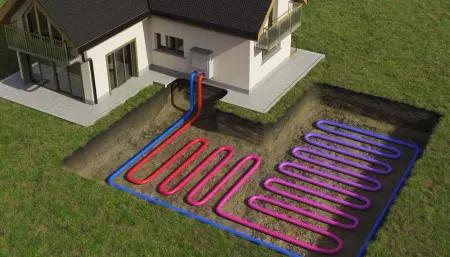
\includegraphics[scale=0.7]{pictures/geoterma-padrao.jpeg}
    \caption{Esquema de construção de geoterma com tubulação enterrada}
    \label{geothermal-default}
    \legend{Fonte: https://pt.solar-energia.net/energia-renovavel/energia-geotermica, acesso em Junho de 2025}
\end{figure}

\begin{figure}[ht]
    \centering
    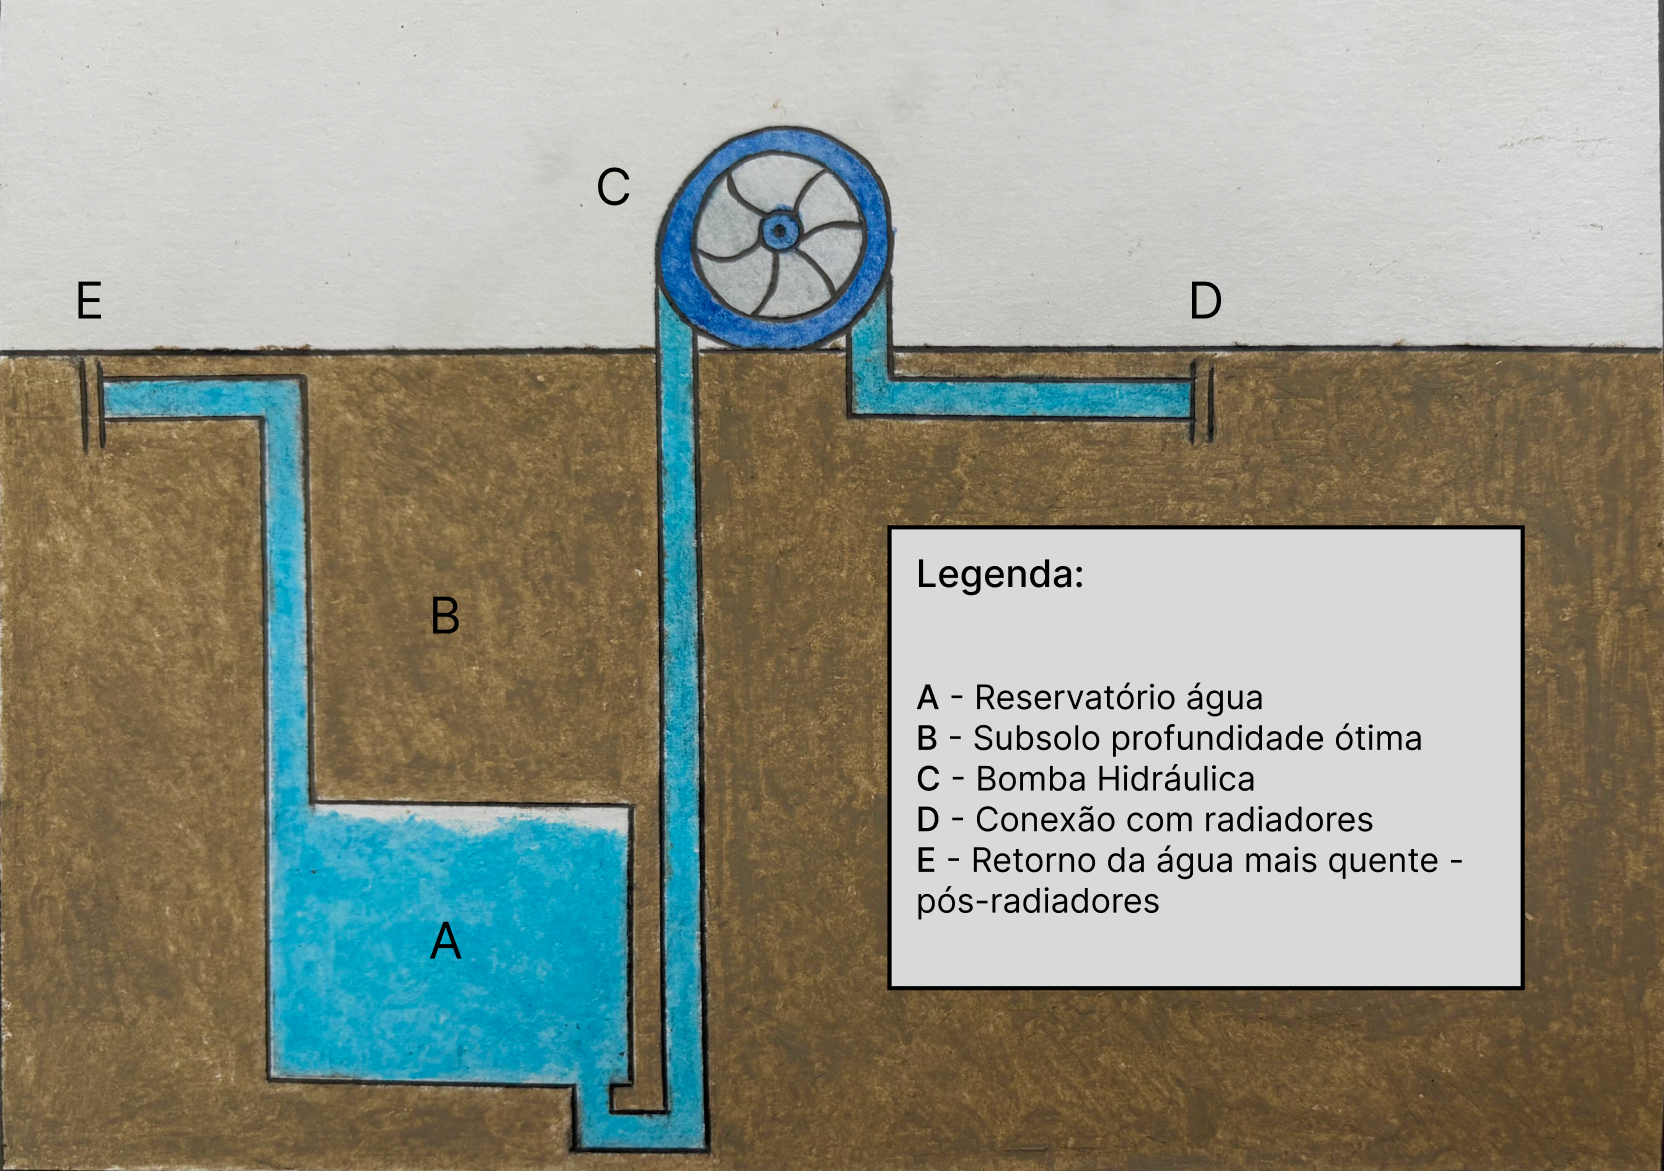
\includegraphics[scale=0.6]{pictures/geoterma.png}
    \caption{Esquema de construção de um poço para refrigeração geotérmica sugerido}
    \label{geothermal-new}
\end{figure}


Essa tecnologia não é benéfica apenas para centros urbanos, pois tem potencial para revolucionar a agricultura. Além de ser possível criar estufas com climatização controlada, é possivel fazer um combate a desertificação com a produção de matéria orgânica e criação de mudas. Portanto, estufas com refrigeração geotérmica atuam no combate à desertificação de múltiplas formas e pode ser a chave para converter terras improdutivas em regiões economicamente autônomas. Porém, para uso em ambientes fechados pode ser necessário o uso de ventiladores atrelados aos radiadores para melhor eficiência em trocas térmicas. Na (\autoref{poste}) exemplifico um uso de radiador ao ar-livre e já na (\autoref{estufa}) é um exemplo para ambiente fechado.

\begin{figure}[ht]
    \centering
    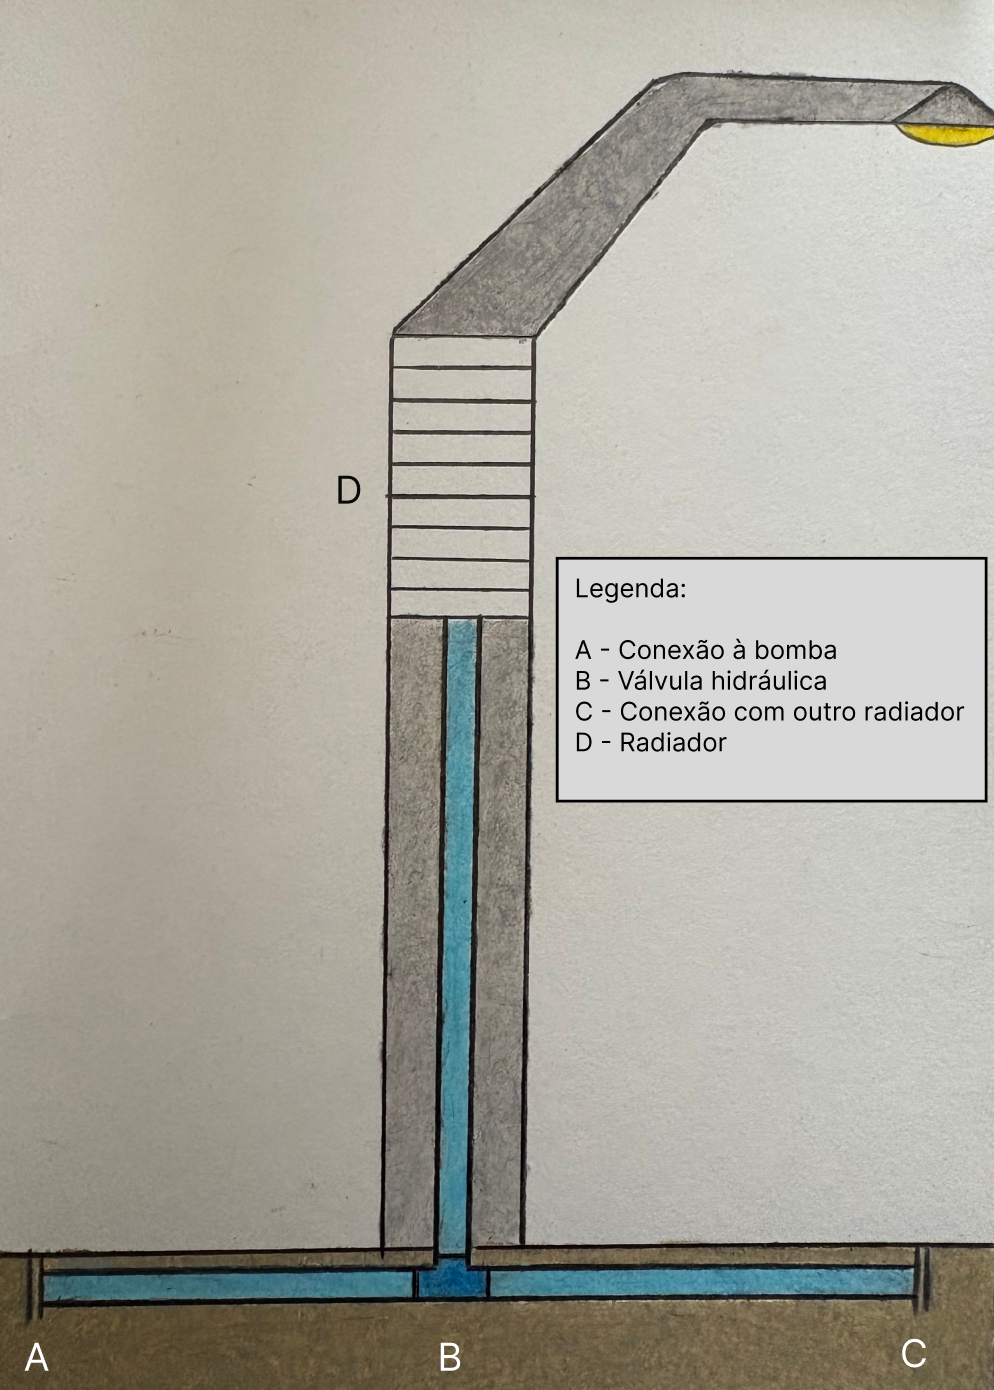
\includegraphics[scale=0.25]{pictures/poste.png}
    \caption{Esquema de construção de um radiador público em um poste}
    \label{poste}
\end{figure}

\begin{figure}[ht]
    \centering
    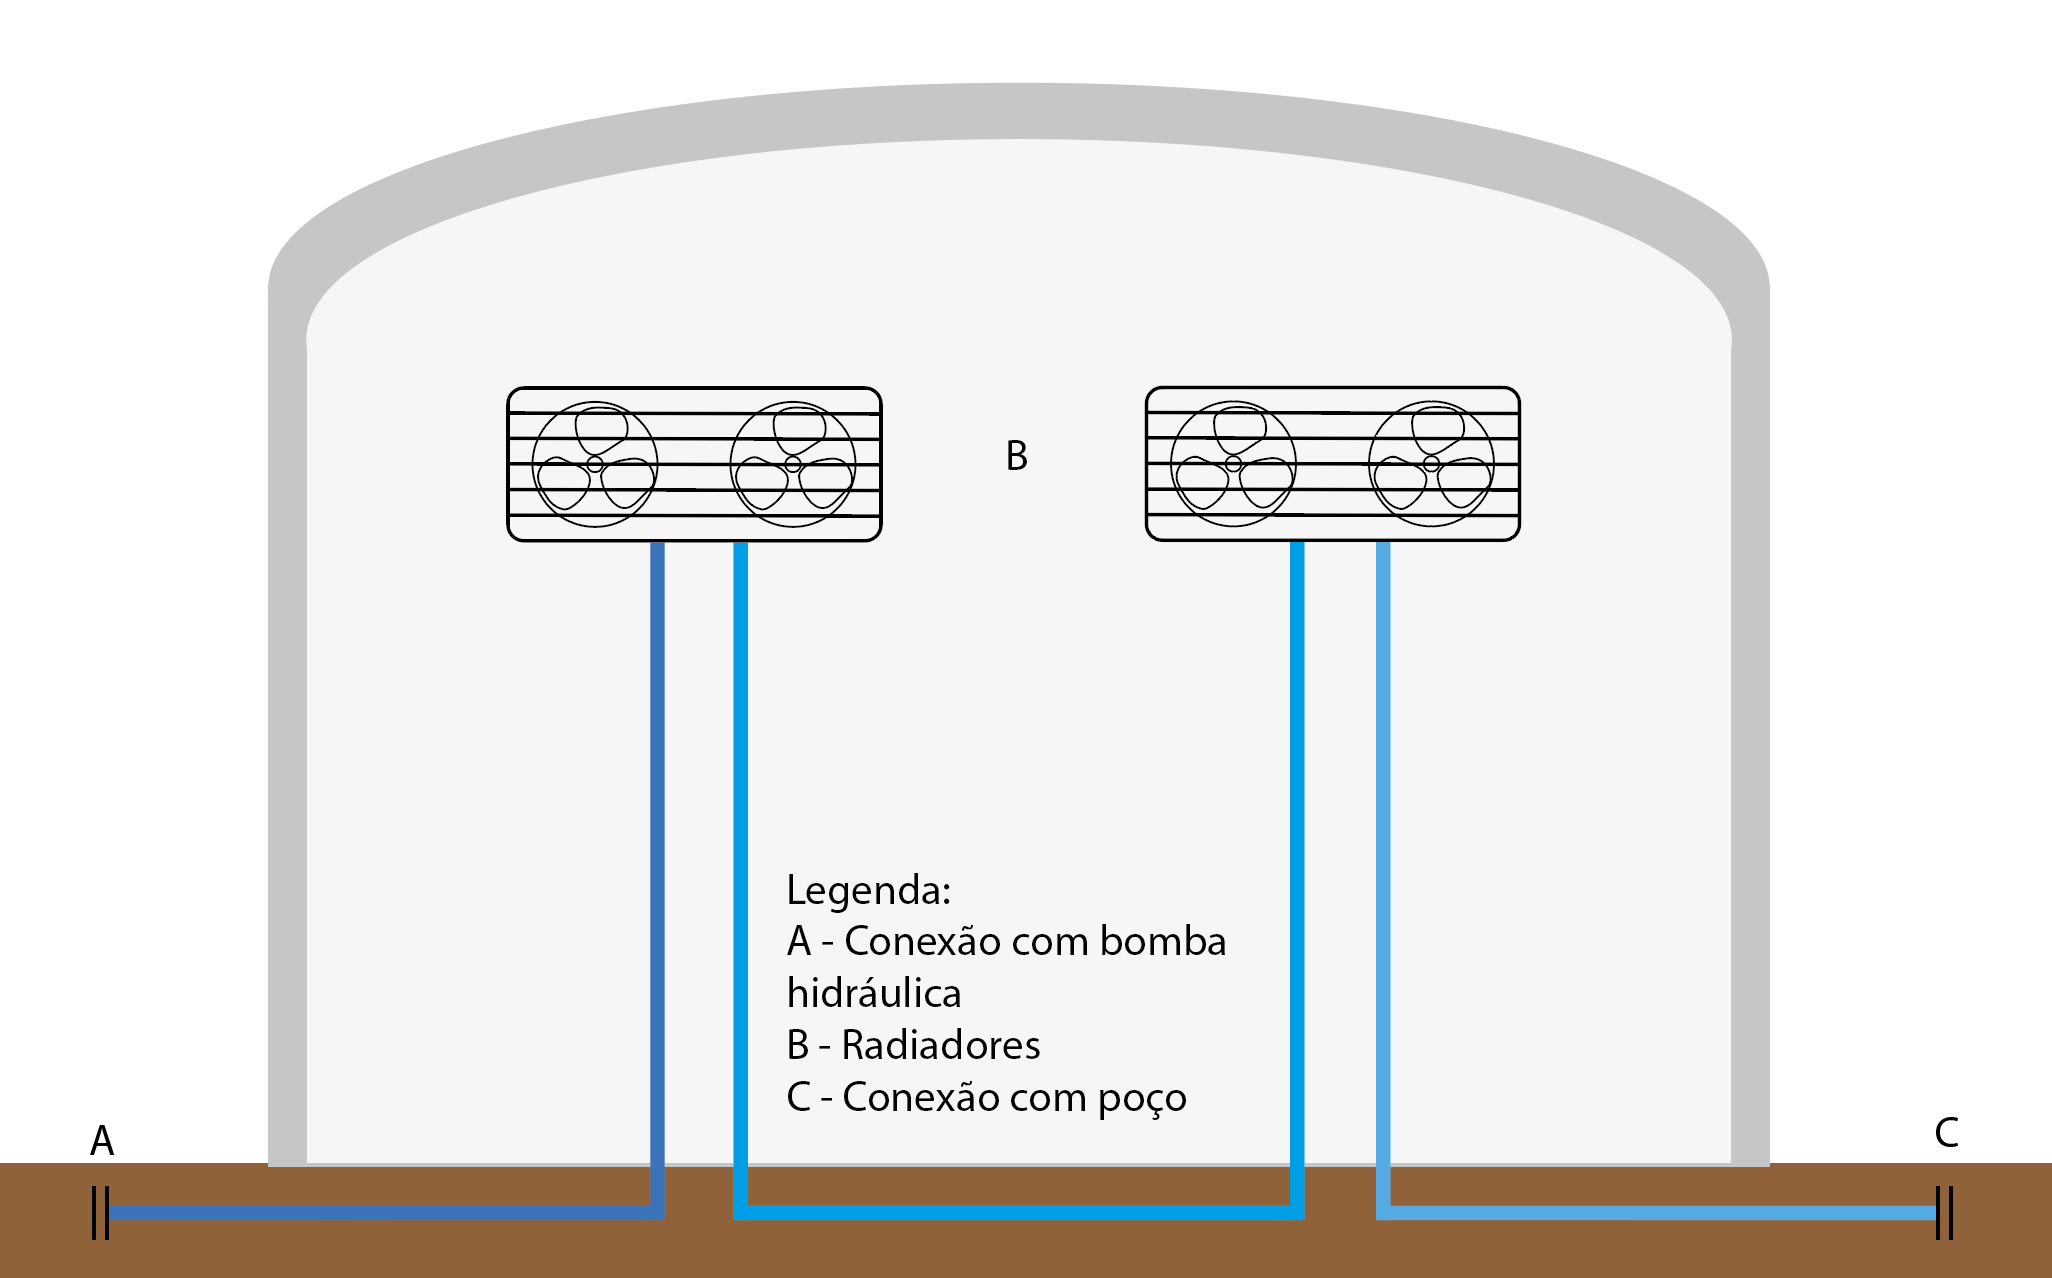
\includegraphics[scale=0.25]{pictures/estufa.png}
    \caption{Esquema de construção de um radiador para ambiente fechado - ex. estufa}
    \label{estufa}
\end{figure}

\section{Experimento}

A tese aqui escrita está em forma puramente teórica e é necessário a criação de um experimento para confirmá-la, deixando sempre bem claro que o desenvolvimento científico deve ser empírico e colaborativo. O experimento proposto é escolher uma região metropolitana com alto uso de ar-condicionados e criar o primeiro refrigerador geotérmico no local. Assim que o refrigerador estiver em funcionamento, é necessário que não se use os ACs e utilize os sistemas de monitoramento meteorológicos para averiguar se o efeito de refrigeração está de acordo com a teoria. Lembrando que ainda não é possível prever quantos sistemas deverão ser construídos para estabilizar a atmosfera terrestre, mesmo se essa teoria estiver válida.

Como já antes mencionado, a temperatura da profundidade ideal para os poços - a qual deve ser em torno de 2m - varia dependendo de diversos fatores como latitude da localização, estação do ano e tipo de solo. Porém, como a quantidade de calor gerada no meio urbano se reduziria com o fim dos ACs, um outro efeito benéfico é que isso seria refletido na temperatura do subsolo com o passar do tempo, ou seja, esse sistema se torna mais eficiente em retirar calor com o passar dos anos.